\documentclass{beamer}
%\documentclass[handout]{beamer}
\usepackage[ngerman]{babel}
\usepackage[utf8]{inputenc}
\usepackage[T1]{fontenc} 
\usepackage{lmodern}

\usepackage{hyperref}


%\usepackage{amsmath, amsthm, amssymb} 
%\usepackage{mathtools}


%\usepackage{listings} 
 \usepackage{color}

 \definecolor{hfugreen}{RGB}{0,136,84}
 \usepackage{tikz}
    \usetikzlibrary{positioning}
    \tikzstyle{rec}=[fill=hfugreen,text=white,
        minimum size=2em, minimum width=9em]

\usepackage{graphicx}


\usetheme{Antibes}
%\usetheme{Luebeck}
%\usecolortheme{seagull}
%\usecolortheme{chameleon}%seagull
\usecolortheme[RGB={0,136,84}]{structure}
\beamertemplatenavigationsymbolsempty

%\mode<presentation>{
%\hypersetup{pdfpagemode=FullScreen}
%}





\setbeamertemplate{footline}
{%
\begin{beamercolorbox}[wd=0.5\textwidth,ht=3ex,dp=1.5ex,leftskip=.5em,rightskip=.5em]{author in head/foot}%
\usebeamerfont{author in head/foot}%
\insertframenumber\hfill\insertshortauthor%
\end{beamercolorbox}%
\vspace*{-4.5ex}\hspace*{0.5\textwidth}%
\begin{beamercolorbox}[wd=0.5\textwidth,ht=3ex,dp=1.5ex,left,leftskip=.5em]{title in head/foot}%
\usebeamerfont{title in head/foot}%
\insertshorttitle%
\end{beamercolorbox}%
}



\newcommand{\cob}{Care-o-bot}
\begin{document}
\newif\ifplacelogo
\placelogotrue
\title{Automatische Kalibrierung eines mobilen Serviceroboters}
\subtitle{}
\author{Jannik Abbenseth}
\institute{Hochschule Furtwangen University, Fakultät für Maschinenbau und Mechatronik
    \and Fraunhofer Gesellschaft, Institut für Produktionstechnik und Automatisierung}
\logo{\ifplacelogo\includegraphics[height=.5cm]{images/hfu_logo.pdf}
\hskip2em
\includegraphics[height=.5cm]{images/ipa_xl}\fi}
\date{20. Februar 2013}
\begin{frame}

\titlepage{}

\end{frame}


\begin{frame}
  \frametitle{Ablauf}
  \tableofcontents[pausesections, hideallsubsections]
\end{frame}


\section{Der \cob}
\label{sec:Der \cob}

\begin{frame}
  \frametitle{Ablauf}
  \tableofcontents[currentsection]
\end{frame}


\bgroup
\setbeamercolor{background canvas}{bg=black}
\begin{frame}[plain]



  %\begin{figure}%[htbp]
    %\centering
  \hspace*{-1.05cm} \includegraphics[width=\paperwidth]{images/cobs}
  %\end{figure}
\end{frame}
\egroup


%\begin{frame}

  %\frametitle{Aufbau des \cob}

  %\begin{figure}[htbp]
    %\centering
    %\includegraphics[height=0.65\textheight]{images/cobs}
    %\label{fig:cobs}
  %\end{figure}
%\end{frame}

\placelogofalse
\begin{frame}
  \frametitle{Komponenten des \cob}
\begin{block}
  {Hardware}
\begin{itemize}
    \pause
    \item Kopf mit drei Kameras \pause
    \item Roboterarm mit sieben Freiheitsgraden \pause
    \item Torso auf mobiler Plattform mit mehreren Freiheitsgraden \pause
  \end{itemize}
\end{block}

\pause

\begin{block}{Software}
  \pause
    \begin{itemize}
      \item Ubuntu \pause
      \item Robot-Operating-System \pause
      \item ROS Nodes
    \end{itemize}
  \end{block}
\end{frame}

\placelogotrue

\placelogofalse
\begin{frame}

  \frametitle{Aufgaben des \cob}

  \begin{block}{Anforderungen an den \cob}
    \pause
    \begin{itemize}
      \item Gegenstände greifen \pause
      \item Niemanden verletzen\pause
      \item Nichts zerstören \pause (auch nicht sich selbst)
    \end{itemize}
  \end{block}
  \pause

  \begin{block}{Lösungen}
    \pause
    \begin{itemize}
      \item Manuelle Bedienung \pause
      \item Autonomes System \pause mit automatischer Kalibrierung
    \end{itemize}
  \end{block}
\end{frame}

\placelogotrue


\begin{frame}
  \frametitle{Ablauf der bisherigen Kalibrierung}
  \setbeamercovered{invisible}

  \onslide*<2>{
    \begin{figure}[htbp]
      \centering
      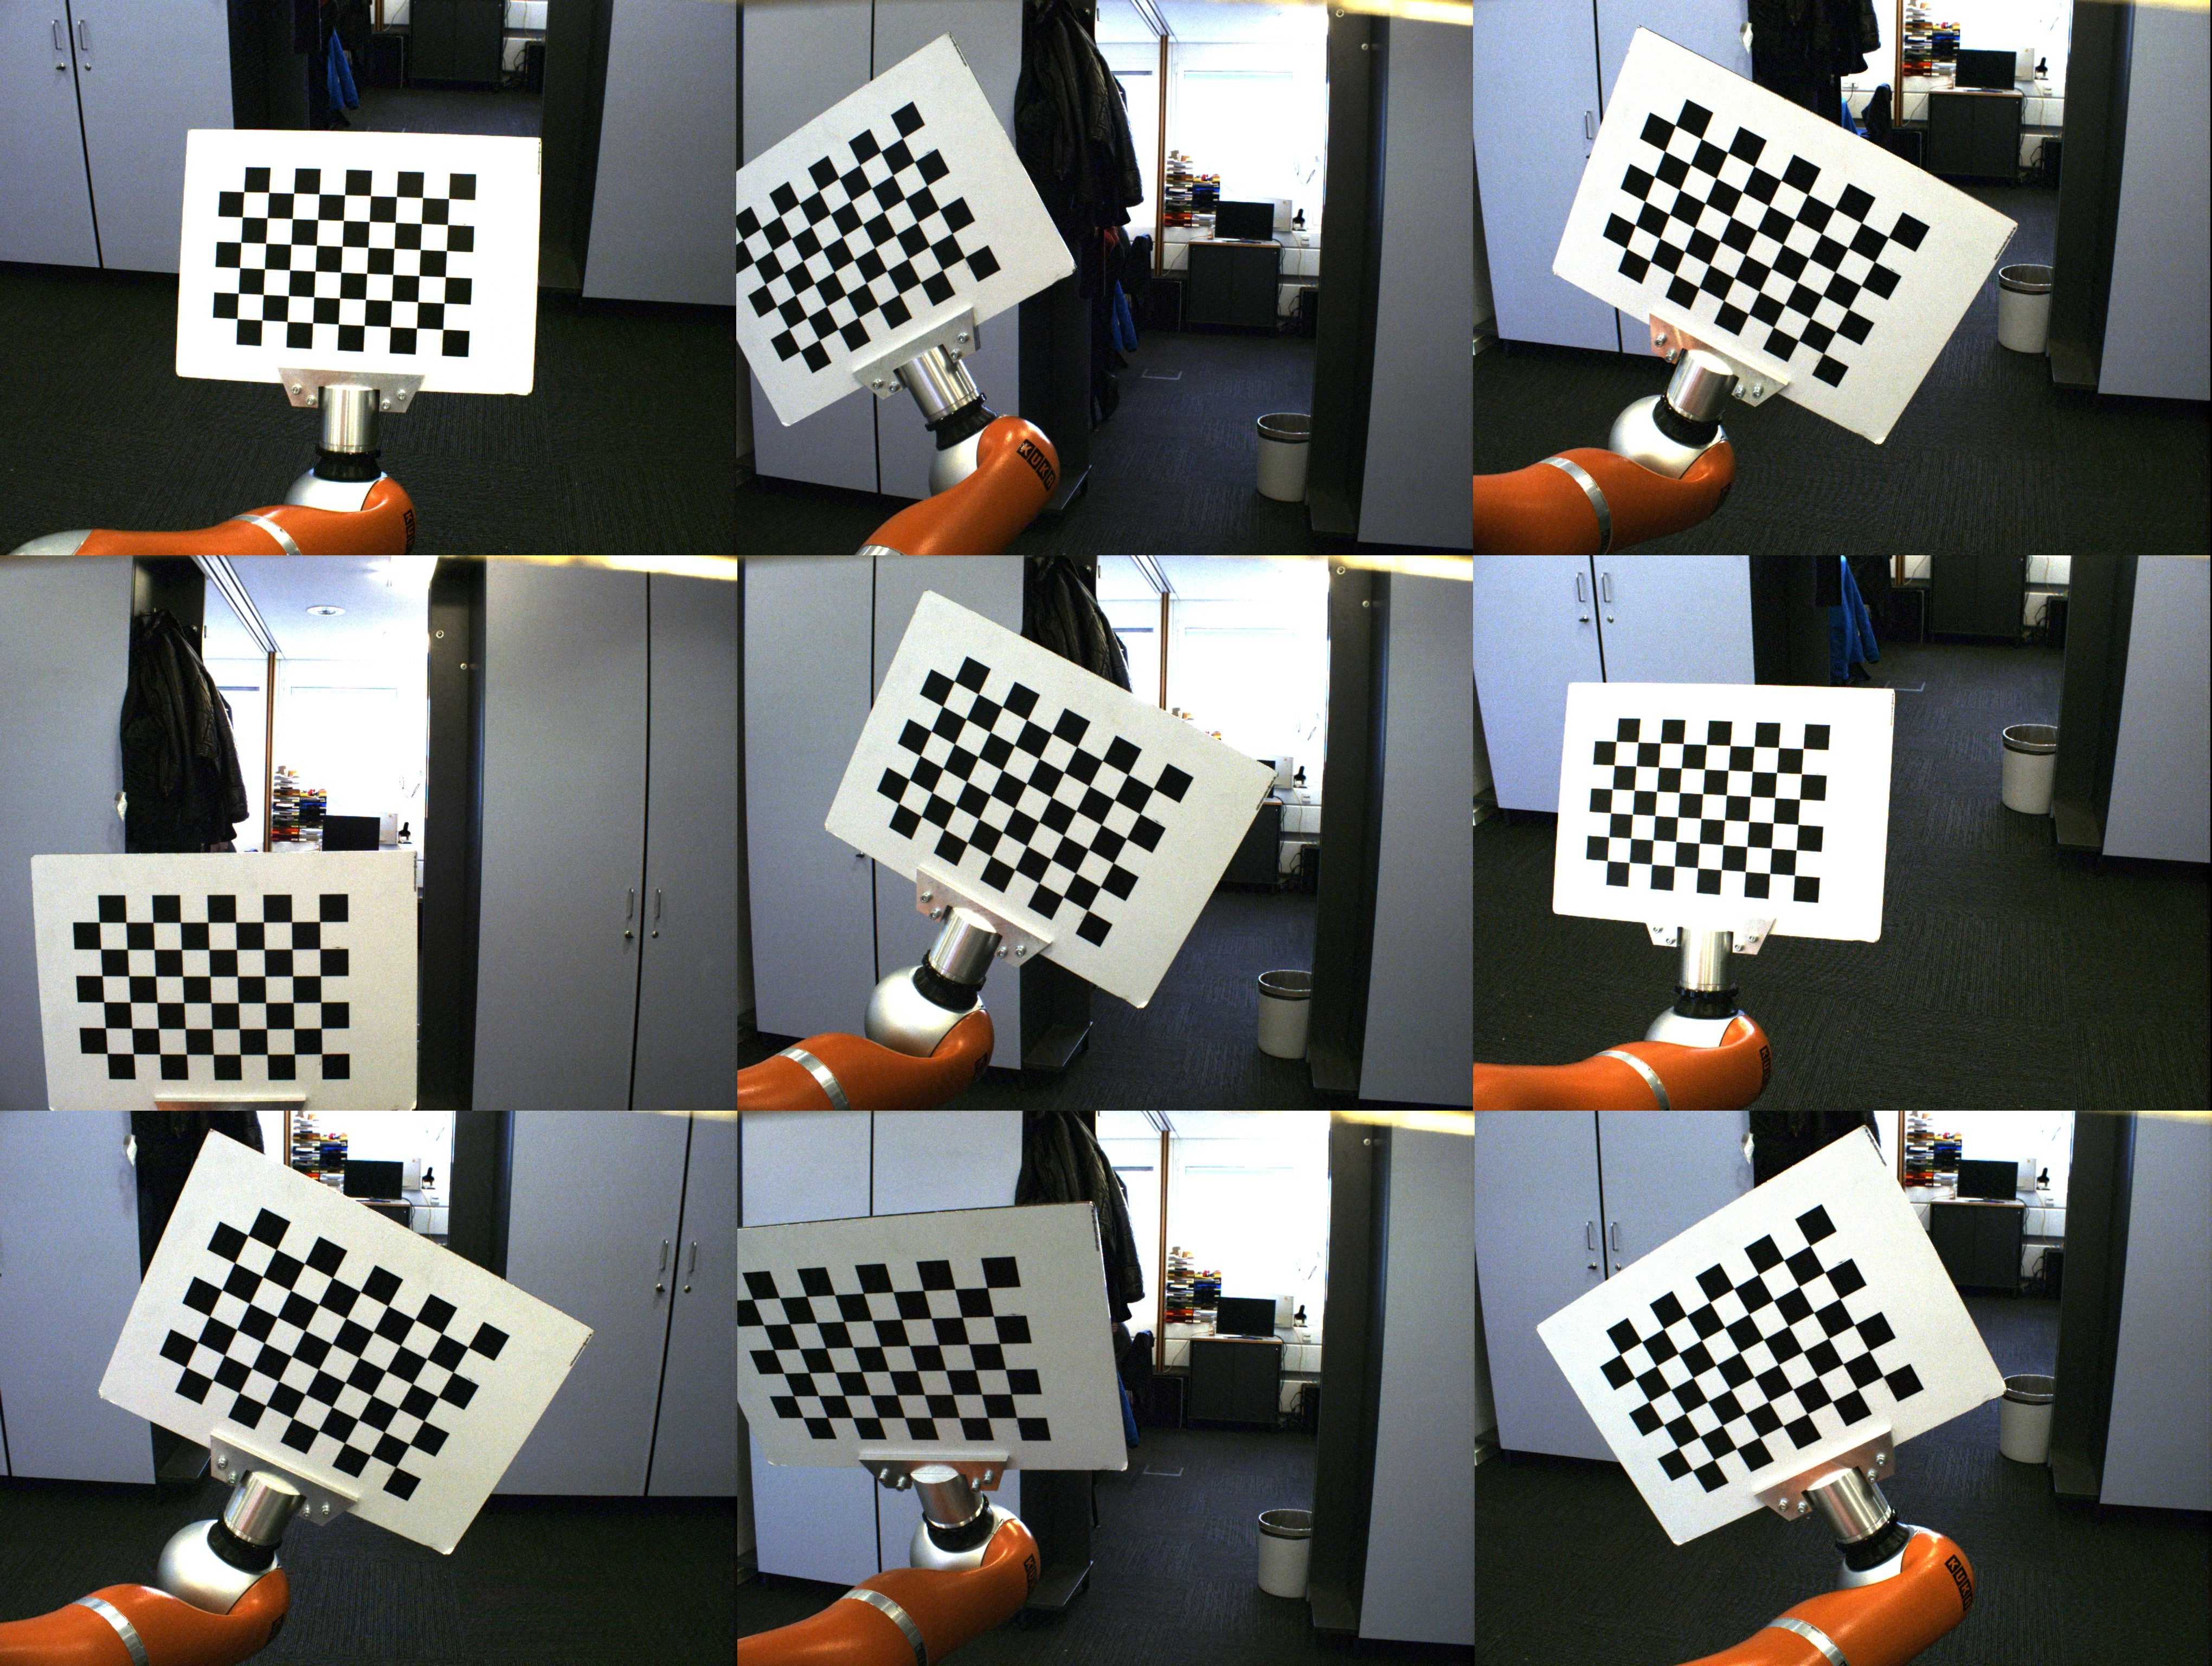
\includegraphics[width=.7\textwidth]{images/calibration_samples}
      \caption{Kalibrierungsbilder}
    \end{figure}
  }

  \onslide<1,3->{
    \begin{center}
      \begin{tikzpicture}[node distance = 2.5em]
        \node(datenaufnahme)[rec]{Datenaufnahme};
          \onslide<3->{ 
        \node (kamerakalibrierung)[rec, below=of datenaufnahme] {Kamerakalibrierung};
        \draw[->] (datenaufnahme) -- (kamerakalibrierung);
      }\onslide<4->{
        \node (datenaufnahme2)[rec, below=of kamerakalibrierung]{Datenaufnahme};
        \draw[<-] (datenaufnahme2) -- (kamerakalibrierung);
      }\onslide<5->{
        \node(kalibrierung) [rec, below=of datenaufnahme2] {Kalibrierung}; 
        \draw[->] (datenaufnahme2) -- (kalibrierung);
      }
    \end{tikzpicture}
  }
\end{center}
\end{frame}

\section{Verbesserungen der automatischen Kalibrierung}
\label{sec:Verbesserungspotential der bisherigen Kalibrierung}


\begin{frame}
  \frametitle{Ablauf}
  \tableofcontents[currentsection,pausesubsections]
\end{frame}
\subsection{Doppelte Modellierung vermeiden}
\begin{frame}
  \frametitle{Doppelte Modellierung des Roboters}

  \begin{block}{Problem}
    \pause
    \begin{itemize}
      \item Roboterbeschreibung in URDF \pause
      \item Beschreibung der Kinematiken in Denavit-Hartenberg Parametern \pause
    \end{itemize}\end{block}
$\rightarrow$ Unnötiger Mehraufwand
\end{frame}

\begin{frame}
  \frametitle{Doppelte Modellierung des Roboters vermeiden}
  \begin{block}{Lösungen}
    \pause
    \begin{itemize}[<+->]
      \item Berechnung der Denavit-Hartenberg Parameter
      \item Nutzung der URDF Beschreibung
      \item \color<5>[rgb]{1,0,0}Abspeichern der Transformation bei der Datenaufnahme
    \end{itemize}\end{block}
\end{frame}



\subsection{Feste Parametrisierung}

\begin{frame}
  \frametitle{Feste Parametrisierung}
  \begin{block}{Anpassungen für den Roboter im Quellcode} \pause
    \begin{itemize}
      \item für jeden Roboter war ein eigenes Build erforderlich \pause
      \item Anforderungen die nicht jeder Roboter erfüllen konnte 
    \end{itemize}\end{block}
\end{frame}

\begin{frame}
  \frametitle{Lösung}
  \begin{block}{Auslagern der Parameter in Konfigurationsdateien} \pause
    \begin{itemize}
      \item Kameradaten \pause
      \item Kalibrierungsobjekt 
    \end{itemize}
  \end{block}
  
    \pause
  \begin{block} {Berechnung der Zielpositionen}
    \pause
    \begin{itemize}
      \item Festlegen eines Bereiches und einer Dichte \pause
      \item Berechnung der Samples \pause
    \end{itemize}
  \end{block}

  $\rightarrow$ Neue Roboter lassen sich einfacher in die Kalibrierung einbeziehen
\end{frame}

\subsection{Doppelte Datenaufnahme vermeiden}

\begin{frame}
  \frametitle{Doppelte Datenaufnahme}
  \begin{block}{Datenaufnahme} \pause
    \begin{itemize}
      \item Datenaufnahme zur Kamerakalibrierung \pause
      \item Datenaufnahme zur kinematischen Kalibrierung \pause
    \end{itemize}
  \end{block}
  \begin{block}{Problem}
    \pause
    \begin{itemize}
      \item Müssen überwacht werden \pause
      \item Zeitaufwendig
    \end{itemize}
  \end{block}
\end{frame}

\begin{frame}
  \frametitle{Lösung}
  \begin{block} {Reduzieren auf einfache Datenaufnahme}
    \pause
    \begin{itemize}
      \item Aufnehmen und speichern von Rohbildern \pause
      \item Kalibrierung der Kameras \pause
      \item Zusätzliche Berechnung der Linsenverzerrung im kinematischen Optimierer \pause
    \end{itemize}
  \end{block}
$\rightarrow$ Schnellere und sicherere Kalibrierung
\end{frame}
  

\section{Ergebnisse und Ausblick}
\begin{frame}
  \frametitle{Ablauf}
  \tableofcontents[currentsection]
\end{frame}


\label{sec:Ergebnisse und Ausblick}

\chapter{Ausblick und Fazit}
utdrianetdriauerneaiudtrneadtrunaifdegpbtdiurneatnsiutaedtrnuaie


%\nocite{*}
%\begin{frame}[allowframebreaks]{Bibliography}
%\printbibliography
%\end{frame}

\end{document}


